\section{Evaluation}
\label{s:eval}

% TODO: Be consistent about machine vs. target.
% Maybe move comparison against P4 to the end of the evaluation.
% Say LOC comparison and qualitatively mention difficulty of implementation.
% Maybe put it at the last.

\begin{table}[!t]
  \begin{scriptsize}
  \begin{tabular}{|p{0.13\textwidth}|p{0.22\textwidth}|p{0.04\textwidth}|}
    \hline
    Atom & Description & Area ($\mu m^2$)\\
    \hline
    Stateless & Arithmetic, logic, relational, and conditional operations on packet/constant operands & 1384 \\
    \hline
    Read/Write & Read/Write packet field/constant into single state variable. & 250 \\
    \hline
    ReadAddWrite (RAW) & Add packet field/constant to state variable (OR) Write packet field/constant into state variable. & 431 \\
    \hline
    Predicated ReadAddWrite (RAW) & Execute RAW on state variable only if a predicate is true, else leave unchanged. & 791 \\
    \hline
    IfElse ReadAddWrite (IfElseRAW) & Two separate RAWs: one each for when a predicate is true or false. & 985 \\
    \hline
    Subtract (Sub) & Same as IfElseRAW, but also allow subtracting a packet field/constant. & 1522 \\
    \hline
    Nested Ifs (Nested) & Same as Sub, but with an additional level of nesting that provides 4-way predication. & 3597 \\
    \hline
    Paired updates (Pairs) & Same as Nested, but allow updates to a pair of state variables, where predicates can use both state variables. & 5997 \\
    \hline
  \end{tabular}
  \end{scriptsize}
  \caption{Atom areas in a 32 nm standard-cell library.  All atoms
  meet timing at 1GHz. Each of the seven compiler targets contains one of the
  seven stateful atoms and the single stateless atom.}
  \label{tab:templates}
\end{table}

\begin{table*}[!t]
  \begin{tabular}{|p{0.16\textwidth}|p{0.43\textwidth}|p{0.08\textwidth}|p{0.06\textwidth}|p{0.07\textwidth}|p{0.03\textwidth}|p{0.03\textwidth}|}
\hline
Algorithm & Description & Least expressive atom & Pipeline depth, width & Ingress or Egress Pipeline? & Domino LOC & P4 LOC\\
\hline
\pbox{0.16\textwidth}{Bloom filter~\cite{bloom}\\(3 hash functions)} & \pbox{0.54\textwidth}{Set membership bit on every packet.} & Write & 4, 3 & Either & 29 & 104 \\
\hline
\pbox{0.16\textwidth}{Heavy Hitters~\cite{opensketch}\\(3 hash functions)} & Increment Count-Min Sketch~\cite{cormode} on every packet. & RAW & 10, 9 & Either & 35 & 192 \\
\hline
Flowlets~\cite{flowlets} & Update saved next hop if flowlet threshold is exceeded. & PRAW & 6, 2 & Ingress & 37 & 107 \\
\hline
RCP~\cite{rcp} & \pbox{0.44\textwidth}{Accumulate RTT sum if\\RTT is under maximum allowable RTT.} & PRAW & 3, 3 & Egress & 23 & 75 \\
\hline
\pbox{0.16\textwidth}{Sampled\\NetFlow~\cite{sampled_nflow}} & \pbox{0.47\textwidth}{Sample a packet if packet count reaches N;\\Reset count to 0 when it reaches N.} & IfElseRAW & 4, 2 & Either  & 18 & 70 \\
\hline
HULL~\cite{hull} & Update counter for virtual queue. & Sub & 7, 1 & Egress & 26 & 95 \\
\hline
\pbox{0.16\textwidth}{Adaptive\\Virtual Queue~\cite{avq}} & Update virtual queue size and virtual capacity & Nested & 7, 3 & Ingress & 36 & 147 \\
\hline
\pbox{0.16\textwidth}{Priority computation for weighted fair queueing~\cite{pifo_hotnets}} & Compute packet's virtual start time using finish time of last packet in that flow. & Nested & 4, 2 & Ingress & 29 & 87 \\
\hline
\pbox{0.16\textwidth}{DNS TTL change tracking~\cite{dns_change}} & Track number of changes in announced TTL for each domain & Nested & 6,3 & Ingress & 27 & 119 \\
\hline
CONGA~\cite{conga} & \pbox{0.54\textwidth}{Update best path's utilization/id if we see a better path.\\
                                           Update best path utilization alone if it changes.}  & Pairs & 4, 2 & Ingress & 32 & 89\\
\hline
%trTCM~\cite{trTCM} & Update token counts for each token bucket & Doesn't map & 7, 3 & Either \\
%\hline
CoDel~\cite{codel} & \pbox{0.54\textwidth}{Update:\\Whether we are marking or not.\\Time for next mark.\\Number of marks so far.\\Time at which min. queuing delay will exceed target.}& Doesn't map & 15, 3 & Egress & 57 & 271\\
\hline
\end{tabular}
\caption{Data-plane algorithms}
\label{tab:algos}
\end{table*}

First, we evaluate \pktlanguage's expressiveness by using it to write several
data-plane algorithms (Table~\ref{tab:algos}), and comparing it to developing
them in P4~(\S\ref{ss:expressive}).  To validate that these algorithms can be
implemented at line-rate, we design a concrete set of \absmachine machines
(Table~\ref{tab:templates}) that we use as compiler targets for
\pktlanguage~(\S\ref{ss:targets}).  We verify that these machines can readily
be implemented in hardware today and that their atoms incur modest chip area
overhead.\footnote{We develop our own atoms since no existing programmable
switching chip supports a sufficiently rich set of operations needed for
data-plane algorithms.} Next, we use the \pktlanguage compiler to compile the
algorithms in Table~\ref{tab:algos} to these targets~(\S\ref{ss:compiler}).  We
conclude by quantifying the tradeoff between a target's programmability (the
space of data-plane algorithms that it can run at line rate) and the target's
performance (the maximum line rate it can support)~(\S\ref{ss:perfprog}).

\subsection{Expressiveness}
\label{ss:expressiveness}

To evaluate \pktlanguage's expressiveness, we program several data-plane
algorithms (Table~\ref{tab:algos}) in \pktlanguage. These algorithms encompass
a variety of data-plane functionality including data-plane load balancing,
in-network congestion control, active queue management, security, and
measurement. In addition, \pktlanguage can be used to program the priority
computation for programming scheduling using the push-in first-out queue
abstraction~\cite{pifo_hotnets}. In all these cases, the algorithms are
naturally available as blocks of imperative code; translating them to
\pktlanguage syntax was straightforward.

By contrast, expressing one of these algorithms in P4 requires manually teasing
out portions of the algorithm that can reside in independent match-action
tables and then chaining these tables together. In essence, the programmer
carries out the transformations in \pktlanguage's compiler. Of the algorithms
in Table~\ref{tab:algos}, only flowlet switching has a publicly available P4
implementation~\cite{p4_flowlet} that we can compare against. This
implementation requires 231 lines of uncommented P4, in comparison to the 37
lines of \pktlanguage in Figure~\ref{fig:flowlet_code}. It also requires the
programmer to manually specify tables, the actions within the tables, how
tables are chained, and what headers are required---all to implement a single
data-plane algorithm. This process can be automated; we have developed a
backend for \pktlanguage that generates P4 code (code counts for these
autogenerated P4 programs are listed in Table ~\ref{tab:algos}).

%%TODO: Decide whether we want to keep this.
%%%Further, the same implementation~\cite{p4_flowlet} is only guaranteed to be
%%%correct on a software switch because it requires synchronized access to the
%%%saved\_hop variable from two adjacent pipeline stages, which requires locking
%%%that is challenging at line rate. This illustrates the additional programmer
%%%burden when programming with P4. Reasoning about how state variables should be
%%%distributed across a pipeline is error prone and is best moved into a compiler
%%%where all algorithms can benefit from it.
%%%
\subsection{Compiler targets}
\label{ss:targets}

We design a concrete set of compiler targets for \pktlanguage based on the
\absmachine machine model. First, we specify computational limits on atoms in
each compiler target using atom templates. Using the Synopsys Design
Compiler~\cite{synopsys_dc}, we quantify the area of each atom's digital
circuit in a 32 nm standard-cell library when running at 1 GHz.  Second, using
an individual atom's area and a switching chip's area~\cite{gibb_parsing}, we
determine the machine's resource limits i.e. the pipeline width for each atom
and the pipeline depth.

\paragraph{Computational limits}
Stateless atoms are easier to design because arbitrary stateless operations can
be spread out across multiple stages of the pipeline without violating
atomicity~(\S\ref{ss:atoms}). We design a stateless atom that can support
simple arithmetic (add, subtract, left shift, right shift), logical (and, or,
xor), relational (>=, <=, ==, !=), or conditional operations ( C's ``?''
operator) on a set of packet fields. Any packet field can also be substituted
with a constant operand.

Designing stateful atoms is more involved because it determines which
algorithms the switch can support. A more complex stateful atom can support
more data-plane algorithms (we show this in the next section), but occupies
greater chip area. To illustrate this, we design a containment hierarchy of
stateful atoms, where each atom can express all stateful operations that its
predecessor can (Table~\ref{tab:templates}).

When synthesized to a 32 nm standard-cell library, all atoms meet timing at 1
GHz and their area increases with the atom's
complexity~(Table~\ref{tab:templates}).

\paragraph{Resource limits}
Now that we have a single stateless atom and multiple stateful atoms, we design
compiler targets using these atoms.  We design one compiler target for each
combination of a stateful atom in Table~\ref{tab:templates} along with the
single stateless atom. We determine resource limits for stateful and stateless
atoms separately.

For the stateless atom, assuming a switch chip's area is 200 $mm^2$ (the
smallest chip area given by Gibb et. al~\cite{gibb_parsing}), and an acceptable
overhead of 7\% (the area overheads for actions in RMT~\cite{rmt}), we can
support ~10000 stateless atoms, given the area of 1384 $\mu m^2$.  This number
is comparable to the 7000 VLIW ALUs supported by RMT~\cite{rmt}, which are
similar in complexity to our stateless atom. If these 10000 atoms were to be
spread across the same number of stages as RMT (30), we could support up to 300
stateless atoms per stage.

A similar analysis for stateful atoms implies around 70 stateful atoms per
stage for the most complex stateful atom with an area of 5997 $\mu m^2$.
However, stateful atoms access memory banks storing state in each stage. The
overhead of providing 70 independent memory banks in each stage supporting one
read and write per clock is prohitibive~\cite{private_conv}. Further, given an
overall stage memory budget, slicing it into many small banks reduces the
amount of memory accessible to each atom. This is problematic for hash-based
algorithms that need to hash into a large memory space. Taken together, these
constraints limit the number of stateful atoms to around 10 per stage, which
greatly reduces their area overhead as well.

In summary, we assume 30 stages in total, 300 stateless atoms per stage and 10
stateful atoms per stage for all compiler targets. By no means is this the only
design. We only claim that this is readily feasible with today's technology and
show that it can be used to implement a wide class of data-plane
algorithms---far beyond a fixed function switch today. As with any
computational substrate, we must start somewhere and refine the instruction set
in response to the algorithms using it.  In a similar vein, designs for
\absmachine machines will evolve as data-plane algorithms demand more of the
hardware.

%We also assume every \absmachine machine provides only one stateful atom
%template, though we don't restrict the number of instances of this template.
%This is because ASIC engineers prefer to design, implement, verify, and
%physically layout one circuit, thereby amortizing design and layout effort over
%multiple instances of the same circuit.

\subsection{Compiling \pktlanguage programs to \absmachine machines}

We now consider every target from Table~\ref{tab:templates}, and every
data-plane algorithm from Table~\ref{tab:algos} to determine if the algorithm
is \textit{implementable} on a particular \absmachine machine. We say an
algorithm is implementable on a \absmachine machine, if every codelet within
the data-plane algorithm can be mapped (\S\ref{ss:code_gen}) to either the
stateful or stateless atom provided by the \absmachine machine. Because
stateful atoms are arranged in a containment hierarchy, we list the
\textit{least expressive} stateful atom/target that can be used to implement a
data-plane algorithm in Table~\ref{tab:algos}. The same table also shows the
algorithms that are implementable on a \absmachine machine with a specific
stateful atom. For instance, a \absmachine machine with the Pairs atom can
implement the first eight algorithms, while a machine with a simpler RAW atom
can implement only the first two.

We note two broader lessons for designing programmable switch chips.  First,
atoms supporting stateful operations on a single state variable are sufficient
for several data-plane algorithms (Bloom Filters through Adaptive Virtual Queue
in Table~\ref{tab:algos}). Second, we find, however, that there are algorithms
that need the ability to update a pair of state variables atomically. One
example is CONGA, whose code we reproduce below:
\begin{verbatim}
  if (p.util < best_path_util[p.src]) {
    best_path_util[p.src] = p.util;
    best_path[p.src] = p.path_id;
  } else if (p.path_id == best_path[p.src]) {
    best_path_util[p.src] = p.util;
  }
\end{verbatim}
Here, \texttt{best\_path} (the path id of the best path for a particular
destination) is updated conditioned on \texttt{best\_path\_util} (the
utilization of the best path to that destination)\footnote{{\tt p.src} is the
  address of the host originating this message, and hence the destination for
the host receiving it and executing CONGA.} and vice versa. These two state
variables cannot be separated into different stages and still guarantee
correctness. The Pairs atom, where the update to a state variable is
conditioned on a predicate of a pair of state variables, allows us to implement
CONGA at line rate.

While the targets in Tab~\ref{tab:templates} are sufficient for several
data-plane algorithms, there are algorithms that they can't run at line rate.
An example is CoDel, which cannot be implemented because it requires a square
root operation that isn't provided by any of our targets. One possibility is a
generic look-up table abstraction that allows us to approximate such
mathematical functions. We leave this exploration to future work.
%%
%%However, it is \textit{still} insufficient for algorithms such as
%%CoDel~\cite{codel} and the two-rate three-color meter (trTCM)~\cite{trTCM}.  On
%%a positive note, however, we observed that the codelets in both trTCM and CoDel
%%are still restricted to a pair of state variables.  We haven't yet encountered
%%a triplet of state variables all falling in the same strongly connected
%%component/codelet, requiring a three-way state update.
%%
\paragraph{Compilation time}
Compilation time is dominated by SKETCH's search procedure.  To speed up the
search, we limit SKETCH to search for constants (e.g., for addition) of size up
to 5 bits, given that the constants we observe within stateful codelets in our
algorithms are small. Our longest compilation time is 10 seconds when CoDel
doesn't map to a \absmachine machine with the Pairs atom because SKETCH has to
search and rule out every configuration in its search space.  This time will
increase if we increase the bit width of constants that SKETCH has to search;
however, because the data-plane algorithms themselves are small, we don't
expect compilation times to be a concern.

\subsection{Performance vs. programmability}
\label{ss:perfprog}
%% \footnote{The compiler only takes
%%clock frequency as a constraint, not an objective to maximize. So, we gradually
%%increase the clock frequency constraint until the compiler fails to meet
%%timing.}
While powerful atoms like Pairs can implement more data-plane algorithms, they
have a cost.  A more expressive atom needs more gates in hardware and incurs
longer signal propagation delays. A longer propagation delay implies a lower
clock frequency (the inverse of propagation delay) and hence a lower line rate.
To quantify this intuition, we consider each stateful atom from
Table~\ref{tab:templates} and synthesize a circuit with the lowest possible
delay using the Synopsys Design Compiler. As we increase the complexity of the
atom, the number of algorithms from Table~\ref{tab:algos} that it can implement
increases (programmability), while at the same time, its achievable line rate
(performance) decreases (Table~\ref{tab:perfprog}).\footnote{The slightly
non-monotonic behavior between PRAW and IfElseRAW is because the logic
synthesis tool is not optimal and employs many heuristics.} This decrease in
line rate can be explained by looking at the simplified circuit diagrams for
the first three atoms (Table~\ref{tab:circuits}), which show an increase in
circuit depth with atom complexity.

\begin{table}[!t]
  \begin{scriptsize}
  \begin{tabular}{|p{0.08\textwidth}|p{0.12\textwidth}|p{0.09\textwidth}|p{0.09\textwidth}|}
  \hline
  Atom & Min. delay (picoseconds) & Programmability (\# of algorithms implemented by atom) & Performance (Max. line rate (Billion pkts/sec)) \\
  \hline
  Write & 176 & 1  & 5.68 \\
  \hline
  ReadAddWrite (RAW) & 316 & 2 & 3.16\\
  \hline
  \pbox{0.1\textwidth}
  {Predicated\\
  ReadAddWrite (PRAW)} & 393 & 4 & 2.54 \\
  \hline
  IfElse ReadAddWrite (IfElseRAW) & 392 & 5 & 2.55 \\
  \hline
  Subtract (Sub) & 409 & 6 & 2.44 \\
  \hline
  Nested Ifs (Nested) & 580 & 9 & 1.72 \\
  \hline
  Paired updates (Pairs) & 609 & 10 & 1.64 \\
  \hline
  \end{tabular}
\end{scriptsize}
\caption{Programmability (the number of algorithms an atom implements)
increases with more complex atoms, but performance (the maximum line rate it
can support in packets / sec) decreases.}
\label{tab:perfprog}
\end{table}

\begin{table}[!t]
  \begin{scriptsize}
    \begin{tabular}{|p{0.08\textwidth}|p{0.28\textwidth}|p{0.05\textwidth}|}
  \hline
  Atom & Circuit & Min. delay in picoseconds \\
  \hline
  Write & 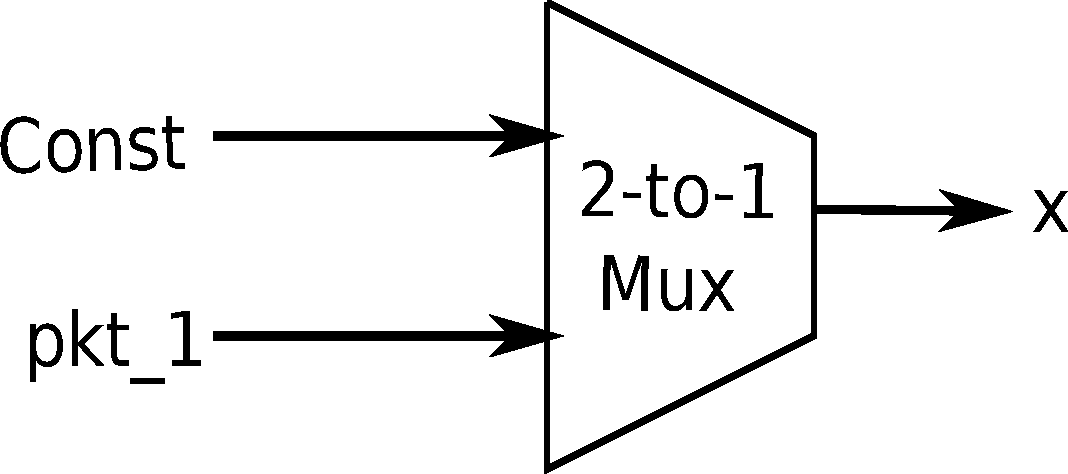
\includegraphics[width=0.2\textwidth]{rw.pdf} & 176 \\
  \hline
  ReadAddWrite (RAW) & 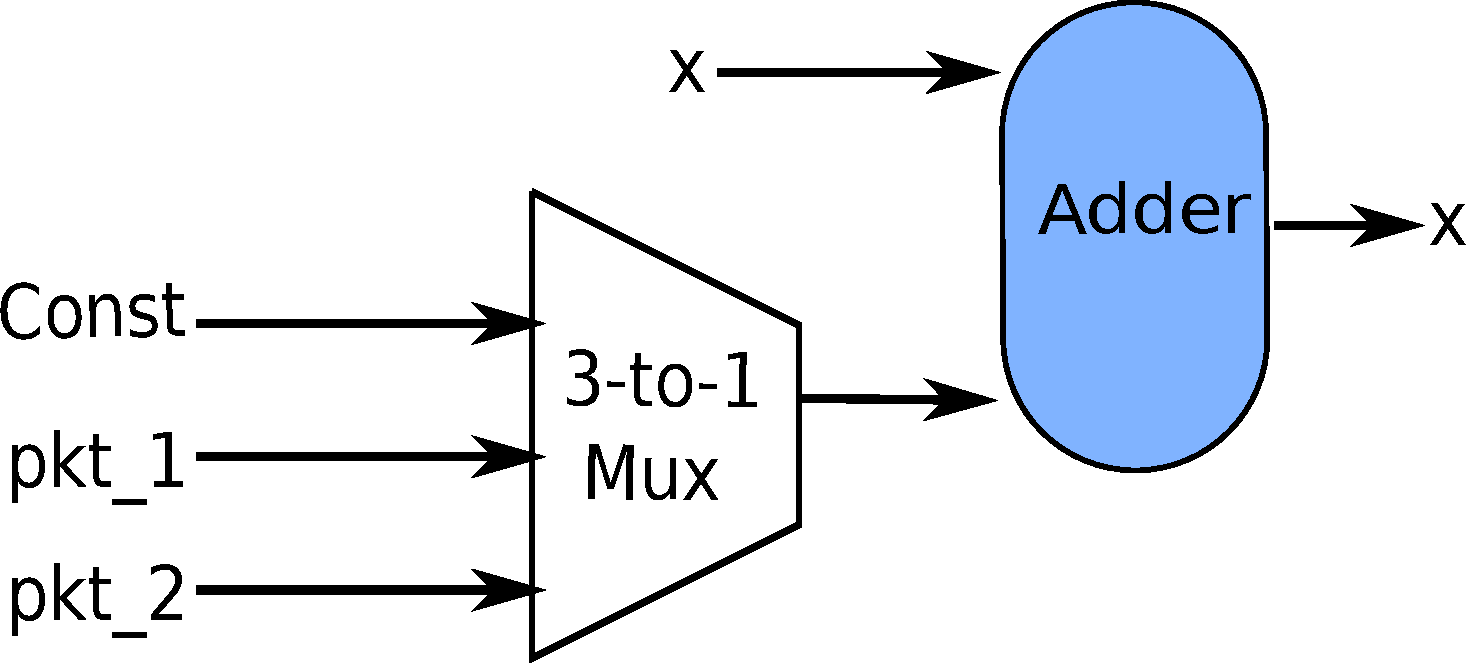
\includegraphics[width=0.2\textwidth]{raw.pdf} & 316\\
  \hline
  \pbox{0.1\textwidth}
  {Predicated\\
  ReadAddWrite (PRAW)} & 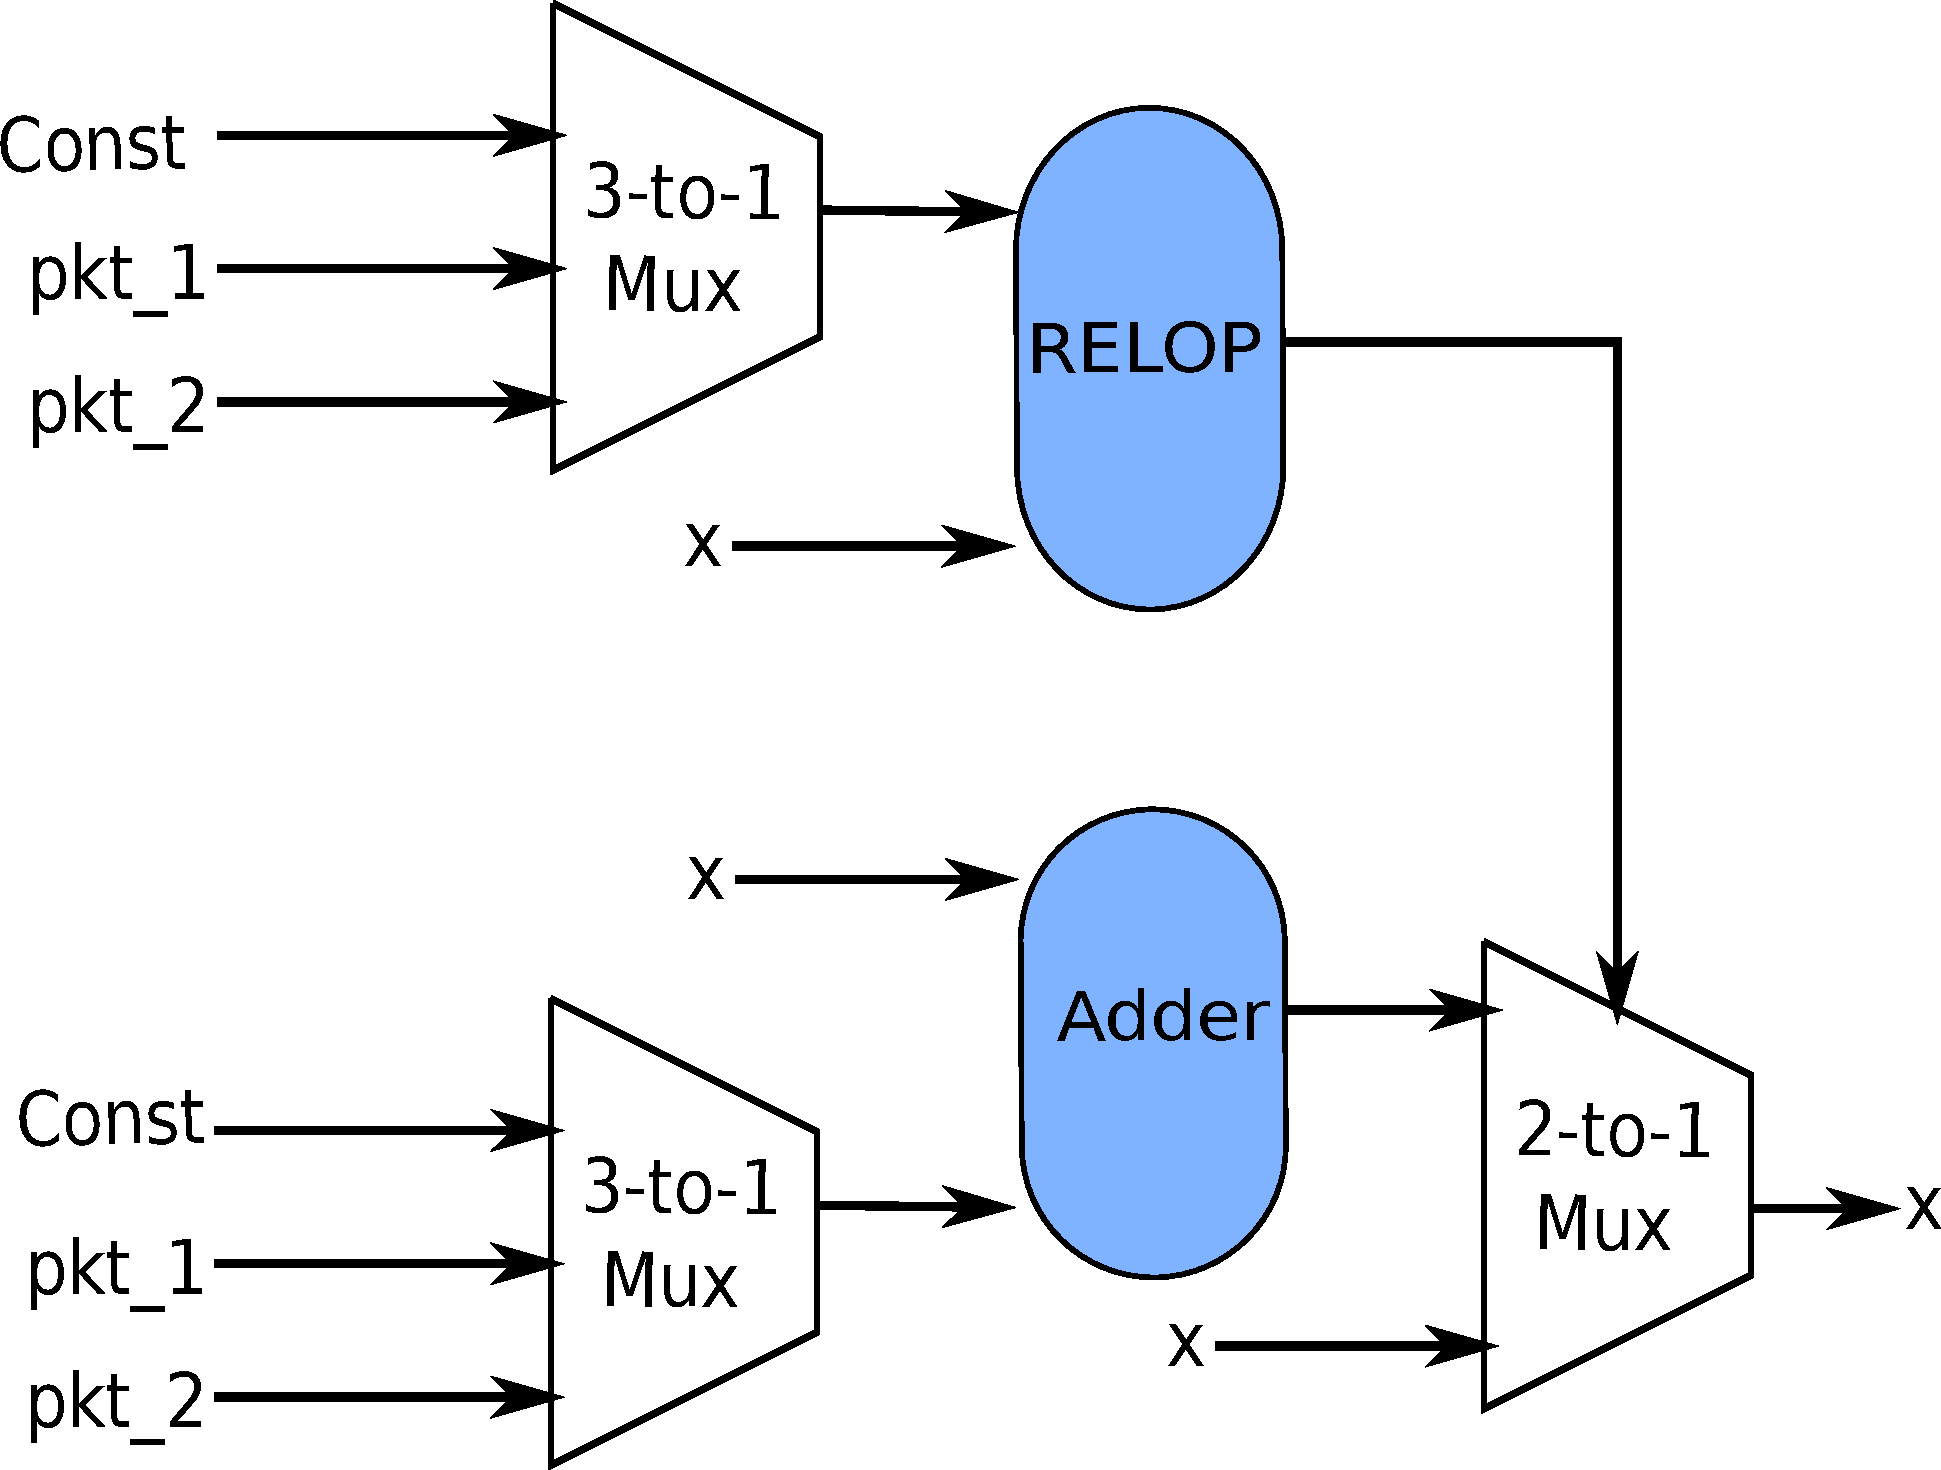
\includegraphics[width=0.3\textwidth]{pred_raw.pdf}  & 393 \\
  \hline
  \end{tabular}
\end{scriptsize}
\caption{Minimum delay of an atom increases with circuit depth. MUX
stands for a multiplexer, RELOP stands for a relational operation between two
operands.}
\label{tab:circuits}
\end{table}
